\scanpage{46}\mspage{45}
de définir une figure $F'$ comme un \uline{\unsure{raffinement|raffinant}} de $F$, si chaque $X'\in F'$ \deleted{\unsure{déf}} est un raffinement d'un $X\in F$. Donc il vaut mieux prendre comme notion primitive celle de \uline{subdivision} d'une \deleted{\unsure{mul|ens}} \inserted{figure}, (qui va se ramener ; celle d'une multistrate), et définir un raffinement d'une figure comme sous-figure d'une subdivision.

Donc, nouveau départ !

Une contrée $C$ est définie par un triple
\[
 (M,\mathcal F,\Sigma)
\]
où $ M$ est un ens (ens. des \uline{multistrates}), $\mathcal F$ un ensemble de parties de $ M$ ($\mathcal F\in\mathcal P(\mathcal P(M))$, \inserted{\unsure{appelées|appelés} \uline{figures},} et $\Sigma$ une relation sur $\mathcal F$ dite : $F'$ \uline{subdivise} $F$. \unsure{Axiomes|Axiome}
% slanted
\margin{Si $F\in\mathcal F$, les $X\in F$ sont les (multi)strates de $F$}

\uline{C 1} Pour tout $X\in M$, $\exists$ \unsure{une|un} plus petite \deleted{partie} figure \deleted{qui} $F_X\unsure{\subset|{,}}$ telle que $X\in F$.

On l'appelle la \uline{figure élémentaire} définie par $X$. On écrit
\[
 X\leq Y\ \overset{\mathrm{def}}{\Longleftrightarrow}\ F_X\subset F_Y\qquad\text{i.e. }X\in F_Y
\]
et on trouve une relation d'\uline{ordre}$^{*}$ $\leq$ sur $ M$.\textsuperscript{$*$}
\margin{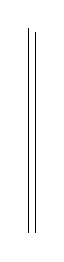
\begin{tikzpicture}\draw (0,0)--(0,2.6);\draw (.09,0)--(.09,2.55);\end{tikzpicture}}
% slanted
\margin{$^{*}$ On veut que ce soit une relation d'ordre \unsure{demander} \unsure{ds|des} ax. \uline{C$'$1} \unsure{pour ça|pour que} si \deleted{\unsure{pr|f}} $X\ne Y$, $\exists$ $F\in\mathcal F$ qui \unsure{contient} \unsure{un des deux} \unsure{ms} $X,Y$, \unsure{et pas l'autre}, \unsure{i.e.} $F_X\ne F_Y$.}
% slanted
\margin{-- i.e. $\mathcal F$ séparé les éléments de $ M$}
